\newcommand{\HSLtag}{\scalebox{1.25}{%
  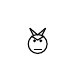
\begin{tikzpicture}
  \draw (0.1,0.2) -- (0.2,0.115) -- (0.3,0.2) ;
  %
  \draw (0.1,0.2) -- (0.15,0.1) ;
  \draw (0.3,0.2) -- (0.25,0.1) ;
  %
  \draw (0.12,0.1) -- (0.2,0.05) -- (0.28,0.1) ;
  %
  \draw (0.2,0) circle (0.12) ; 
  \draw (0.16,0.04) circle (0.01) ;
  \draw (0.24,0.04) circle (0.01) ;
  \draw (0.15,-0.07) -- (0.25,-0.07) ;
  \end{tikzpicture}
}}

\newcommand{\HSLbox}{\rule{1ex}{1ex}}

\newcommand{\HSL}[1][]{\vbox{\medskip\noindent\hrulefill \\[5pt]
  \HSLtag \hspace{\stretch{1}}HIC SUNT
  LEONES \; {#1}\hspace{\stretch{1}} \HSLtag \\ \smallskip\noindent\hrulefill \\}}


%%% If/then check for empty strings (requires xifthen for \ifempty)
\newcommand{\ifempty}[3]{%
  \ifthenelse{\isempty{#1}}{#2}{#3}%
}

\def\negcaptionspace{\vspace{-10pt}}

%\newcommand{\mypar}[1]{\paragraph*{#1}}
\newcommand{\mypar}[1]{\medskip\noindent\textbf{#1.}}
\newcommand{\myparB}[1]{\noindent\textbf{#1.}  }

\newenvironment{nscenter}
 {\parskip=0pt\par\nopagebreak\centering}
 {\parskip=2pt\par\noindent} % \ignorespacesafterend

\usepackage{refcount}
\newcommand{\myfootnotemark}{\footnotemark\label{fn:mark}}
\newcommand{\myfootnotetext}[1]{\footnotetext{#1\label{fn:text}%
        \edef\fnmark{\getpagerefnumber{fn:mark}}%
        \edef\fntext{\getpagerefnumber{fn:text}}%
        \ifx\fnmark\fntext\else\ClassWarning{}{footnote mark and text on different pages!}\fi}}

\newcommand{\codefont}{\fontsize{10}{10}\selectfont}
\newcommand{\code}[1]{{\tt\codefont {#1}}}
\newcommand{\smallcode}[1]{{\tt\codefont\footnotesize {#1}}}
\newcommand{\contract}[1]{{\tt\codefont{\txColor{#1}}}}
\newcommand{\txcode}[1]{{\text{\tt\codefont{\txColor{#1}}}}}
\newcommand{\smalltxcode}[1]{{\text{\tt\codefont\footnotesize{\txColor{#1}}}}}

\newcommand{\solcode}[1]{\lstinline[language=solidity]{#1}}
\newcommand{\cvlcode}[1]{\lstinline[language=cvl]{#1}}

\newcommand\bslash{\symbol{`\\}}
\def\etc{\emph{etc}.\@\xspace}
\newcommand{\Eg}{E.g.\@\xspace}
\newcommand{\eg}{e.g.\@\xspace}
\newcommand{\ie}{i.e.\@\xspace}
\newcommand{\cf}{cf.\@\xspace}
\newcommand{\wrt}{w.r.t.\@\xspace}

% \newcommand{\argmax}{\operatornamewithlimits{argmax}}
% \newcommand{\argmin}{\operatornamewithlimits{argmin}}
% \renewcommand{\algorithmicrequire}{\textbf{Input: }}
% \renewcommand{\algorithmicensure}{\textbf{Output: }}

\newcommand{\wei}{\textit{wei}\xspace}
\newcommand{\ether}{\textit{ETH}\xspace}
\newcommand{\USD}{\mbox{\textit{USD}}\xspace}
\newcommand{\USDfmt}[1]{\SI[round-precision=0,round-mode=places]{#1}}

\newcommand{\nocheckmark}{}

\newcommand{\keyterm}[1]{\textbf{\emph{#1}}}%

%%%%
% \newmdenv [linewidth=0pt]{mdNoFramed}
%with no line number
\newcommand{\inputJava}[1]{%[backgroundcolor=LightGrey]	
\begin{mdNoFramed}
	\inputminted[%
	fontsize=\footnotesize,%
	%frame=single,%
	%framesep=1.5\fboxsep,%
	%rulecolor=\color{listingFrame}%
	]{solidity}{#1}%
	%\vspace{-2mm}%
\end{mdNoFramed}
}%

%with line number
\newcommand{\inputJavaLinenos}[1]{%
\begin{mdNoFramed}
	%\vspace{1mm}%
        \inputminted[%
       	linenos,
	fontsize=\footnotesize,%
	%frame=single,%
	%framesep=1.5\fboxsep,%
	%rulecolor=\color{listingFrame}%
	]{solidity}{#1}%
	%\vspace{-2mm}%
\end{mdNoFramed}
}%

%with line number  starting at the last line used
\newcommand{\inputJavaLinenosStarting}[1]{%
\begin{mdNoFramed}
	%\vspace{1mm}%
        \inputminted[%
        firstnumber=last, %the last line number used
	linenos,
	fontsize=\footnotesize,%
	%frame=single,%
	%framesep=1.5\fboxsep,%
	%rulecolor=\color{listingFrame}%
	]{solidity}{#1}%
	%\vspace{-2mm}%
\end{mdNoFramed}
}%
\newcommand{\lineno}[1]{{\tt\codefont {\textcolor{magenta}{#1}}}}

%%%%%%%%for iterating on graph
\def\gainList{{Government,EthereumPyramid,ProtectTheCastle,TreasureChest,ZeroPonzi,Ethstick,Doubler2,DynamicPyramid},
              {Etheramid1,LittleCactus,GreedPit,Doubler,ShinySquirrels1,Thesimplegame,Newponzi,Doubler3},
              {Quick1,Myscheme,Bunny,DoubleTx,Multi33v,DianaEthereum-x18,Rubixi}}

\def\ratioList{{Government,EthereumPyramid,ProtectTheCastle,TreasureChest,ZeroPonzi,Ethstick,Doubler2,DynamicPyramid},
              {Etheramid1,LittleCactus,GreedPit,Doubler,ShinySquirrels1,Thesimplegame,Newponzi,Doubler3},
              {Quick1,Myscheme,Bunny,DoubleTx,Multi33v,DianaEthereum-x18,Rubixi}}


\newcounter{gainListCounter}

% \def\colorTx{\color{ForestGreen}}
\def\txColor{\color{MidnightBlue}}
\def\fieldColor{\color{Plum}}
\newcommand{\txFmt}[1]{{\txColor{\sf #1}}}

\newcommand{\tx}[2][]{\txFmt{#2}_{\txColor{#1}}}
\newcommand{\txT}[1][]{\tx[#1]{T}} % transaction
\newcommand{\txTi}[1][]{\txFmt{T'_{\txColor{{\it #1}}}}}
\newcommand{\txTii}[1][]{\txFmt{T''_{\txColor{{\it #1}}}}}

\def\pmvColor{\color{red}}
\newcommand{\pmvFmt}[1]{{\pmvColor{\tt #1}}}
\newcommand{\pmv}[2][]{\pmvFmt{#2}_{\pmvColor{#1}}\xspace}
\newcommand{\pmvA}[1][]{\pmv[{#1}]{A}} % user constant
\newcommand{\pmvB}[1][]{\pmv[{#1}]{B}}
\newcommand{\pmvC}[1][]{\pmv[{#1}]{C}}

\DeclareMathSymbol{:}{\mathord}{operators}{"3A}
\def\tokColor{\color{magenta}}
\newcommand{\tokFmt}[1]{{ \mathtt{\tokColor{#1}} }}
\newcommand{\tok}[2][]{\tokFmt{#2}_{\tokColor{#1}}\xspace}
\newcommand{\tokT}[1][]{\tok[{#1}]{T}}
\newcommand{\tokTi}[1][]{\tok[{#1}]{T'}}

%%% Macros for UTXO Transactions

\def\fieldColor{\color{Plum}}
\newcommand{\txTag}[3][]{{\fieldColor\sf #3}\ifempty{#1}{\ifempty{#2}{}{: {#2}}}{[{#1}]\ifempty{#2}{}{: {#2}}}}

\newcommand{\txIn}[2][]{\txTag[{#1}]{#2}{in}}
\newcommand{\txWit}[2][]{\txTag[{#1}]{#2}{wit}}
\newcommand{\txOut}[2][]{\txTag[{#1}]{#2}{out}}
\newcommand{\txSigned}[2][]{\txTag[{#1}]{#2}{signed}}
\newcommand{\txAfterAbs}[2][]{\txTag[{#1}]{#2}{absLock}}
\newcommand{\txAfterRel}[2][]{\txTag[{#1}]{#2}{relLock}}
\newcommand{\txf}{\txTag{}{f}} % transaction field
\newcommand{\txarg}[1][]{\txTag{}{arg_{#1}}}
\newcommand{\txscript}{\txTag{}{script}}
\newcommand{\txstorage}{\txTag{}{data}}
\newcommand{\txval}{\txTag{}{value}}

% arg fields for token txs
\newcommand{\tkop}{\txTag{}{op}}
\newcommand{\tkown}{\txTag{}{owner}}
\newcommand{\tkval}{\txTag{}{tkval}}
\newcommand{\tkid}{\txTag{}{tkid}}

\newcommand{\const}[2][]{#2_{#1}} % constants
\newcommand{\constK}[1][]{\const[{#1}]{k}}
\newcommand{\constPK}[1][]{\const[{#1}]{pk}}
\newcommand{\constSK}[1][]{\const[{#1}]{sk}}
\newcommand{\constKi}[1][]{\const[{#1}]{k'}}
\newcommand{\constT}[1][]{\const[{#1}]{t}}
\newcommand{\constTi}[1][]{\const[{#1}]{t'}}
\newcommand{\constTii}[1][]{\const[{#1}]{t''}}

% signature verification in the Bitcoin script language
\newcommand{\sig}[3][]{\mathit{sig}^{#1}_{#2}\ifempty{#3}{}{({#3})}}
\newcommand{\versigName}{{\sf versig}}
% \newcommand{\versig}[2]{\versigName({#1},{#2})}
\newcommand{\versig}[2]{\versigName:{#1}}
\newcommand{\rtx}{{\sf rtx}}
\newcommand{\hashE}[1]{{\sf H}(#1)}
\newcommand{\hashSem}[1]{\ifempty{#1}{H}{H(#1)}}
% todo: remove \after
%\newcommand{\after}[2]{\ensuremath{\textsf{after}~{#1}:{#2}}}
\newcommand{\afterAbs}[2]{{\sf absAfter}~{#1}:{#2}}
\newcommand{\afterRel}[2]{{\sf relAfter}~{#1}:{#2}}
\newcommand{\op}[3]{\ensuremath{#2~\textsf{#1}~#3}}
\newcommand{\opSem}[3]{\ensuremath{#2~\mathit{#1}~#3}}
\newcommand{\notE}[1]{{\sf not}~{#1}}
\newcommand{\notSem}[1]{\mathit{not}~#1}
\newcommand{\sizeE}[1]{\ensuremath{| #1 |}}
\newcommand{\ifE}[3]{\mathsf{if}~{#1}~\mathsf{then}~{#2}~\mathsf{else}~{#3}}
\newcommand{\ifSem}[3]{\mathit{if}~{#1}~\mathit{then}~{#2}~\mathit{else}~{#3}}
\newcommand{\ifTSem}[3]{\mathit{if}~{#1}~\mathit{then}~{#2}}
\newcommand{\andE}{~{\sf and}~}
\newcommand{\orE}{~{\sf or}~}
\newcommand{\versigP}[3]{{\sf versig}_{#1}({#2},{#3})}


\newcommand{\usecase}[1]{\emph{#1}}
% \newcommand{\spec}[1]{\textcolor{blue}{\textit{#1}}}

\newcommand{\nexts}{\ensuremath{\mathrm{next}}\xspace
}
\newcommand{\state}[1][]{%
    \ifthenelse{\equal{#1}{}}{\ensuremath{\mathrm{s}}}{\ensuremath{\mathrm{#1}}}%
    \xspace
}
\newcommand{\method}[1][]{%
    \ifthenelse{\equal{#1}{}}{\ensuremath{\mathrm{T}}}{\ensuremath{\mathrm{#1}}}%
    \xspace
}
\newcommand{\Prop}{\ensuremath{\mathrm{P}}}

\newcommand{\user}[1]{\emph{#1}}
